% !TEX root = ../main.tex
\documentclass[../main.tex]{subfiles}
\begin{document}
\label{sec:results}

In this Section we explore the consistency with which volunteers modelled galaxies, the variance of the aggregate model recovered and how well our recovered models agree with other results in the literature.


\subsection{Examination of Volunteer consistency}
We aggregate two independent models for a set of 98 galaxies based on ``original'' or repeat (``validation'') classifications, obtained with the same retirement limit (see Section \ref{sec:retirement-limit} for more on this selection).

One of the simplest choices the volunteers have is whether to include a model component or not. Figure \ref{fig:volunteer_component_consistency} illustrates the consistency with which volunteers made use of a component in their model for a galaxy. We see that volunteer classification is very consistent (scatter in fraction of 0.1), with volunteers almost always using a disc and bulge, and consistent proportions agreeing on the presence of a bar and the number of spiral arms.

\begin{figure*}
  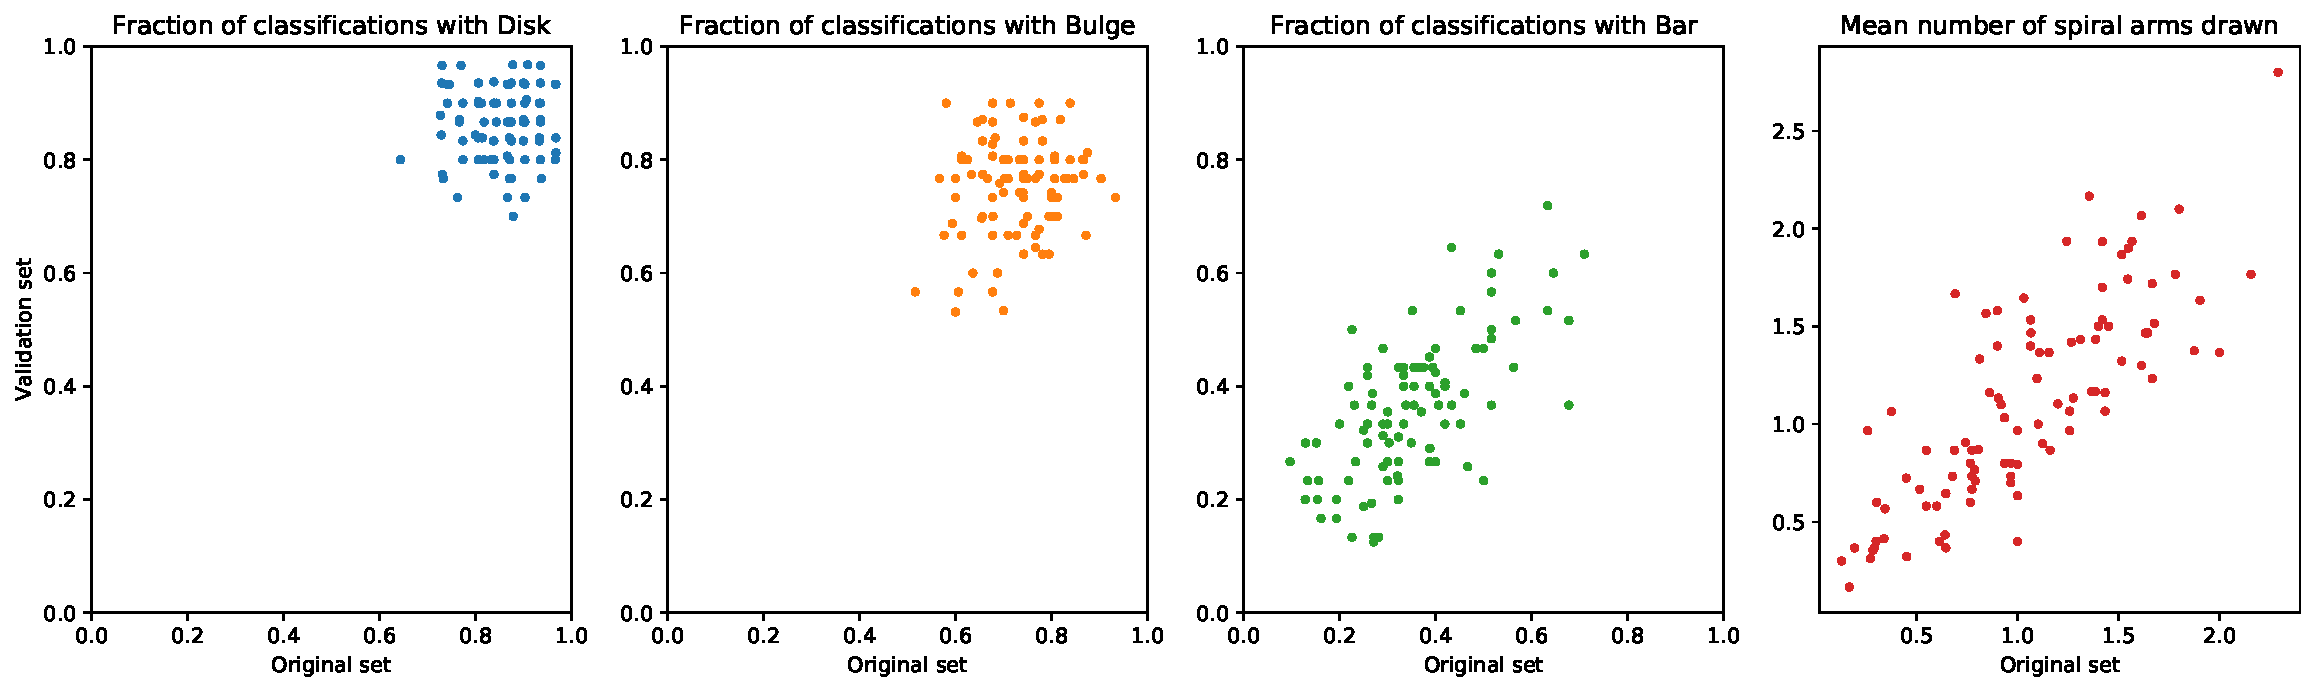
\includegraphics[width=17.3cm]{images__results/component_frequency.pdf}
  \caption{Comparison of frequency of use of component in volunteer models between the original and validation sets of classifications.}
  \label{fig:volunteer_component_consistency}
\end{figure*}

After selecting a component, the volunteer sets its shape and size. We see good consistency in isophotal shape and size, as shown in Figure \ref{fig:aggregate_model_consistency}. The least consistent component is the bar, which may be caused by the lower proportion of volunteers incorporating one into their model. Visual inspection suggests that many volunteers used a very elliptical bulge and drawn spirals to capture the light from the bar. Fewer bars having been drawn by volunteers also has the effect of making clustering more difficult and more uncertain, even for a strongly barred galaxy we effectively go from receiving 30 classifications to around 12 for the bar

\begin{figure*}
  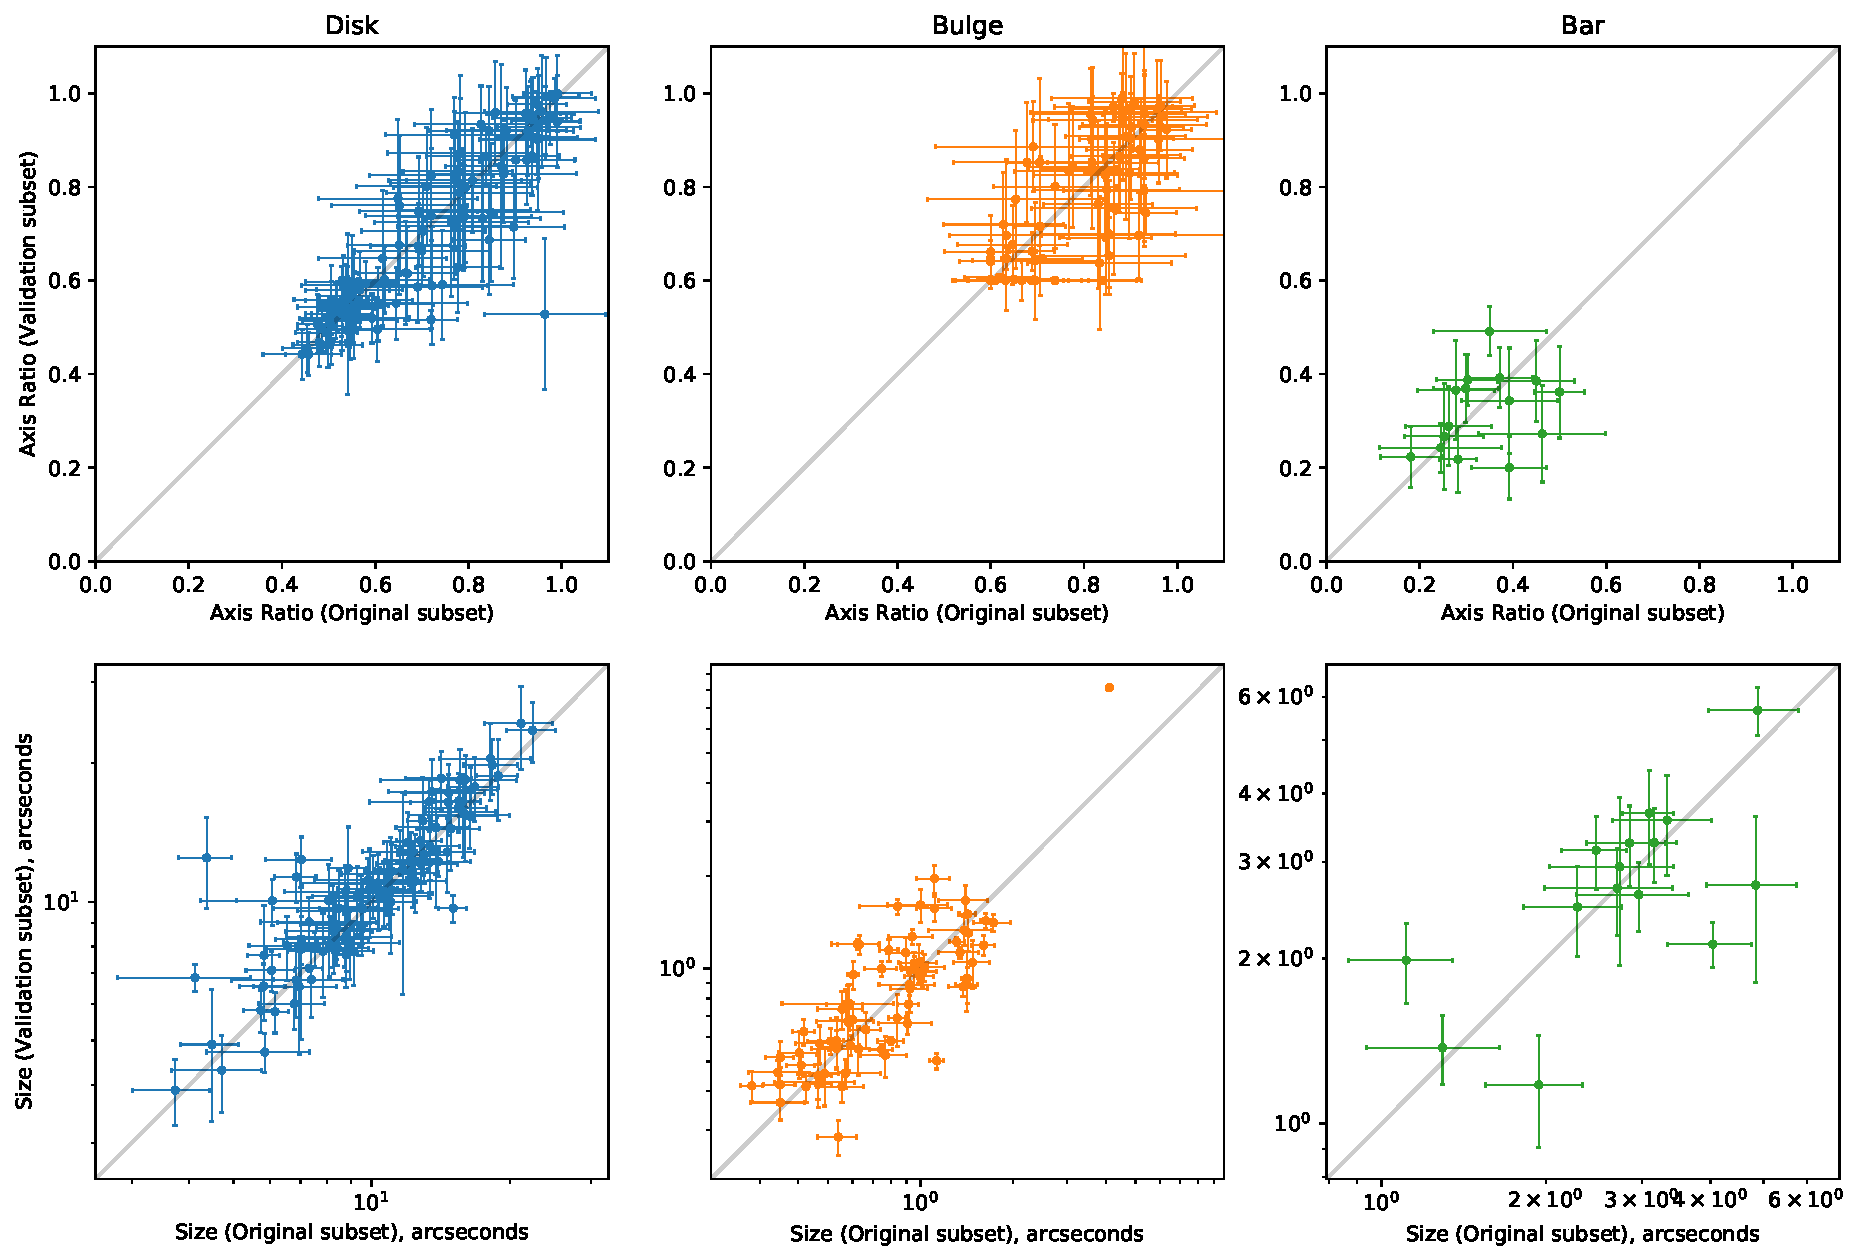
\includegraphics[width=17.3cm]{images__results/component_sizing.pdf}
  \caption{Comparison of component shape in aggregate models between the original and validation sets.}
  \label{fig:aggregate_model_consistency}
\end{figure*}

\subsection{Best Individual vs Aggregate Model}

For each galaxy in the sample we compare the tuned aggregate model to the tuned best individual model, and find that the best individual model consistently outperforms the aggregate (around 70\% of the time). However, there is a very small (less than a 5\%) probability that any individual classifier will beat the aggregate model for more than half of the galaxies they model, with most volunteers outperforming the aggregate less than one in ten times. In summary, for an individual galaxy it is usually the case that the best individual model is best, but these models come from a wide variety of users, not a small number of super-users. It is notable how close many volunteers' models came to the optimial solution without any tuning.

Our recommendation is to make use of the tuned aggregate model for scientific analysis, though users may wish to instead make use of a number of volunteer models as starting points for their own numerical fits.
%if sufficient computation time is available it is likely that the best results can be obtained by using a number of volunteer models as starting points for numerical fits.

\subsection{Comparison to results in the literature}

After having obtained aggregated models for our galaxies, we examine how our models compare to other results in the literature. There exists no published comparison sample with four-component fits, so we are only able to do this separate components (or pairs of components).

We also make comparisons to existing measures of morphology for individual galaxies: When comparing the probability of a classification containing a bar component against a galaxy being classed as strongly-barred or as having no bar (as defined in \citealt{Masters2010:1003.0449v2}), we see a significant difference: classifications of strongly-barred galaxies ($p_\text{bar} > 0.5$) had a $0.47 \pm 0.14$ chance of containing a bar, vs $0.30 \pm 0.11$ for galaxies classed as having no bar ($p_\text{bar} < 0.2$). The Spearman correlation between GZ2's $p_\text{bar}$ and the bar likelihood in \textit{Galaxy Builder} is $0.56$, which implies a significant correlation.

\subsubsection{Comparison to One-component fit - axis ratio}
We compare the axis ratios of the discs recovered from \textit{Galaxy Builder} to the axis ratio of a 2D S\'ersic fit to the r-band SDSS image of each galaxy (as provided in the NASA-Sloan Atlas). We see excellent agreement (Figure \ref{fig:ax_ratio_comparison}), with an error of $\sim0.1$, consistent with our expected errors (derived in Section \ref{sec:error_estimation}). We observe a large number of measurements outside $2\sigma$ around a \textit{Galaxy Builder} axis ratio of 0.5, which is likely to be due to the drawing tool ellipse having a default axis ratio of $0.5$, and biasing volunteer classification or aggregate shapes.

\begin{figure}
  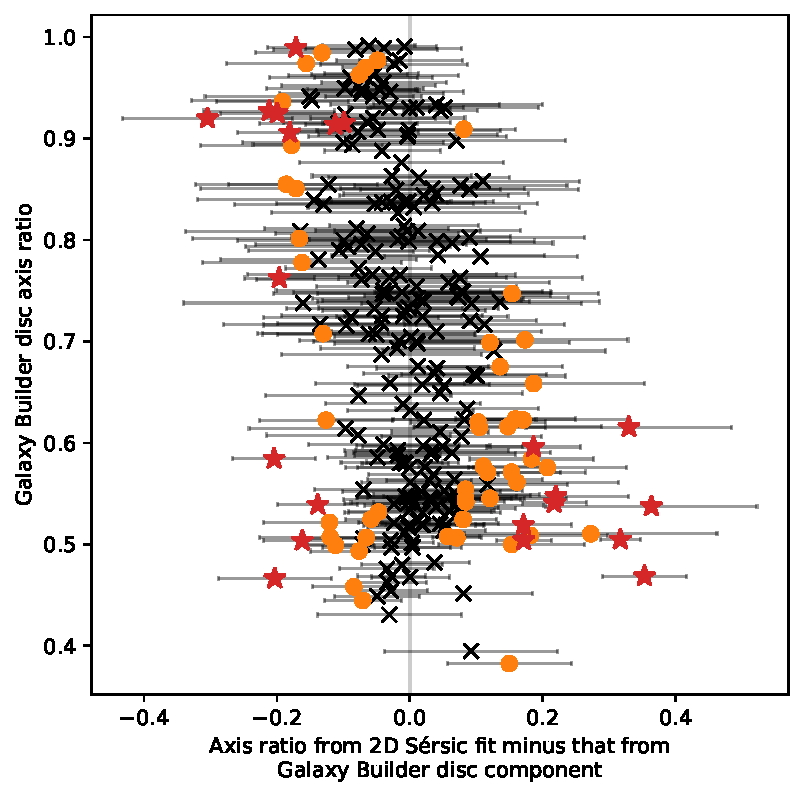
\includegraphics[width=8cm]{images__results/gzb-agg-nsa-comparison.pdf}
  \caption{Difference between the axis ratios of the disc components of aggregated Galaxy Builder models to the results of an r-band S\'ersic profile fit. Points outside 1- and $2\sigma$ are highlighted in orange and red.}
  \label{fig:ax_ratio_comparison}
\end{figure}


\subsubsection{Comparison to Disc-Bulge models}

One of the largest catalogs of 2D many-component fits is \citet{Simard2011:1107.1518v1}, which performed simultaneous, two-bandpass decompositions of 1,123,718 galaxies in the Legacy area of the SDSS DR7 using \textsc{Gim2D}. Three variations of models were fitted: a pure S\'ersic model, an exponential disc and de-Vaucouleurs bulge model, and an exponential disc and a S\'ersic bulge model. \citet{2012MNRAS.421.2277L} similarly fitted two models to SDSS main-sample galaxies: an exponential disk and exponential bulge (\textit{exp+exp}), and an exponential disk and de Vaucouleurs bulge (\textit{exp+dV}). They used a Levenberg-Marquadt gradient descent algorithm, with initial parameters taken from previous SDSS analysis.

Comparing between these catalogues and to \textit{Galaxy Builder} models, we see that our models show excellent agreement with others, where such agreement is to be expected. Comparing bulge to total fraction, we see closest agreement to the \textit{exp+exp} model, where bulge S\'ersic index is similar to that most often chosen by \textit{Galaxy Builder} volunteers (who consistently preferred to use bulges with low S\'ersic indices), as bulge measurements are very sensitive to central substructure and model choice \citep{Gao2017:1709.00746v1}. The Kendall rank correlation coefficients between our measurments and \citet{Simard2011:1107.1518v1} and \citet{2012MNRAS.421.2277L} can be seen in Figure \ref{fig:bt_correlation}. The low correlation coefficients in general, even when comparing the results of fitting identical models (the two \textit{exp+dV} models), further show the difficulty of calculating reliable bulge to total ratios for galaxies. \textit{Galaxy Builder} models agree with more conventional photometrically fit models as well  as those models agree with each other.

% Talk about bias (only 1:1 agreement with exp+exp)?

\begin{figure}
  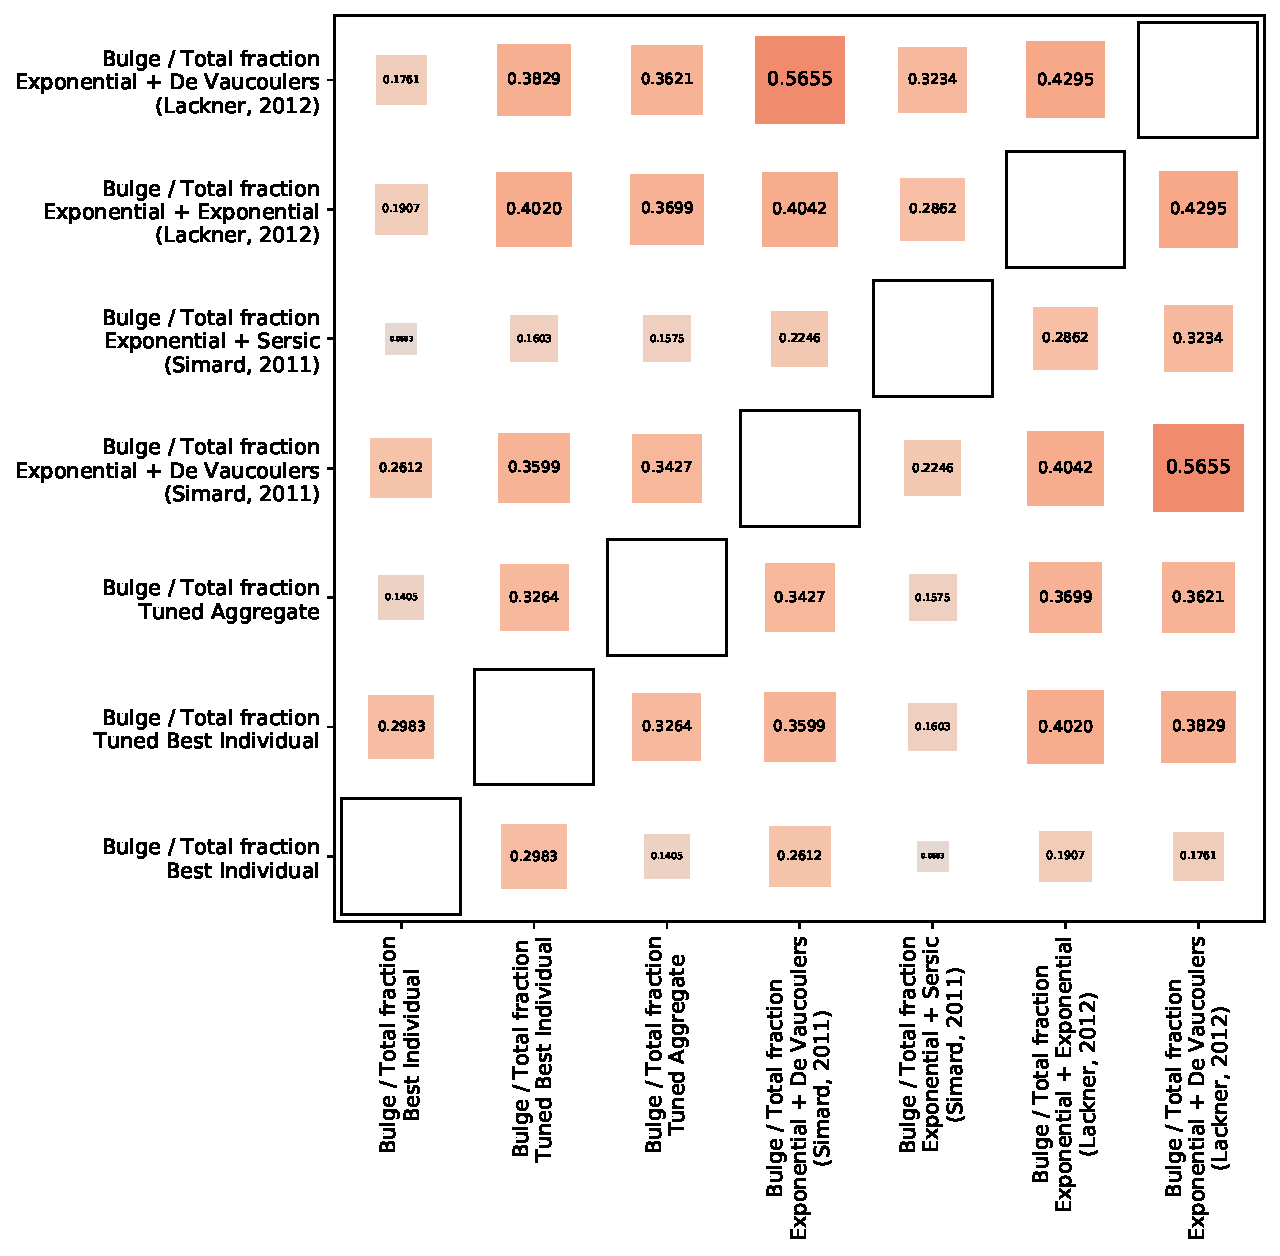
\includegraphics[width=8cm]{images__results/b-t_comparison_correlation.pdf}
  \caption{Correlation matrix showing Kendall rank correlation coefficient between measures of Bulge to Total fraction from \textit{Galaxy Builder} results and other models fitted in \citet{Simard2011:1107.1518v1} and \citet{2012MNRAS.421.2277L}. Colours and box size indicate the strength of the correlation.}
  \label{fig:bt_correlation}
\end{figure}


\subsubsection{Comparison to Disc-Bulge-Bar models}

\citet{Kruk2017:1710.00093v2} performed many-component, multi-band decompositions of a selection of Sloan galaxies, 12 of which were also classified in \textit{Galaxy Builder}. For each of these galaxies we obtain the ``best'' model provided by volunteers (scored using mean squared error, in units of nanomaggies) and futher optimize the slider parameters available to volunteers, as well as the effective radius and axis ratio of all components. Figure \ref{fig:sd_comp_comparison} compares the axis ratios and effective radii of bulges, discs and bars in \citet{Kruk2017:1710.00093v2} to those produced here. We see excellent agreement in effective radius, but a large scatter in axis ratio (though an overall correlation). We do note that galaxy builder bulges generally have a larger effective radius than the bulges in \citet{Kruk2017:1710.00093v2}. This discrepancy could be caused by the differences in bulge S\'ersic index, as bulges present in \citet{Kruk2017:1710.00093v2} tend to have lower S\'ersic indices than those in the \textit{Galaxy Builder} models.


\begin{figure}
  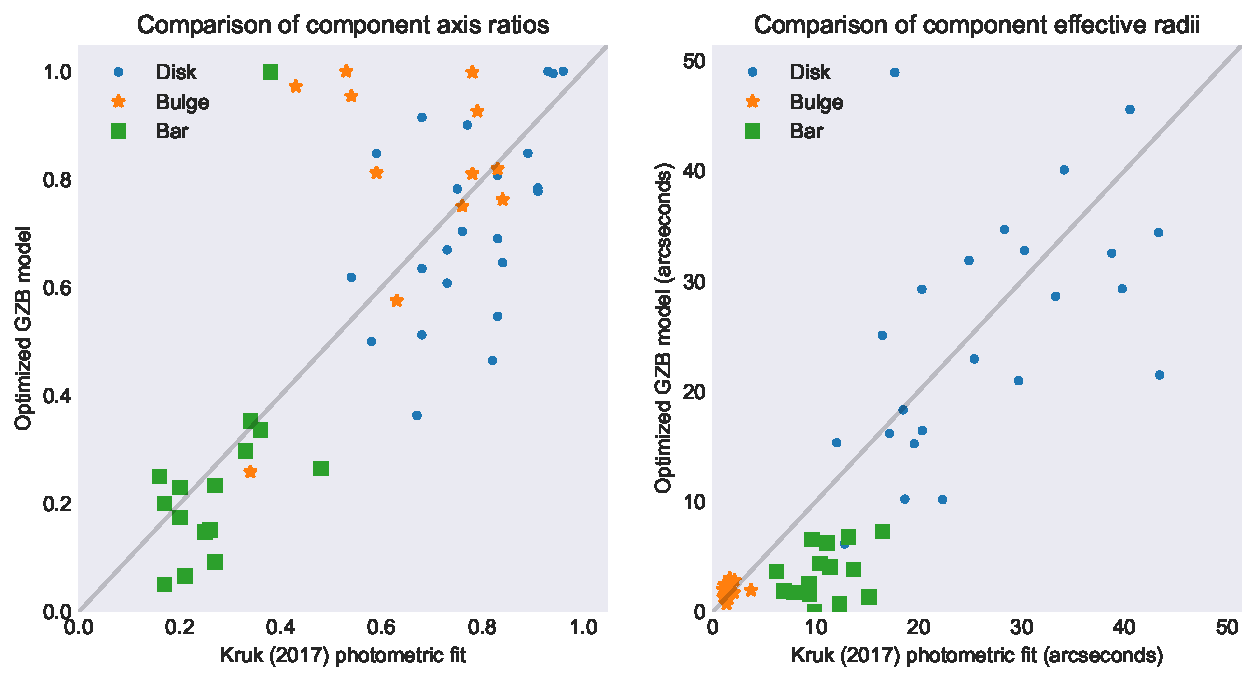
\includegraphics[width=8cm]{images__results/sd_comp_comparison.pdf}
  \caption{Comparison between \textit{Galaxy Builder} tuned aggregate models and the result of 3\-component, multi\-wavelength fits performed by \citet{Kruk2017:1710.00093v2}.}
  \label{fig:sd_comp_comparison}
\end{figure}


\subsubsection{Comparison to Disc-Bulge-Bar-Spiral models}
To the best of our knowledge, no photometic models exist for the Galaxy Builder sample which contain spiral arm structure. The closest comparable result is that produced by \citet{Gao2017:1709.00746v1}, however galaxies used are not in the Sloan footprint.

In order to provide a comparison for our novel method of spiral parameter (pitch angle and amplitude) extraction, we compare the result of our logarithmic spiral fit to the relationship obtained by \citet{Hart2016:1607.01019v1} between GZ2 classification and galaxy pitch angle (Figure \ref{fig:hart_pitch_angle}). Their fit was obtained by using the Zooniverse to filter good vs bad spiral arm segments identified using a leading automated spiral arm detection and fitting tool, \textsc{SpArcFiRe} \citep{Davis2014:1402.1910v1}. We find good agreement; although there are large error bars on the GZ2-produced pitch angle, this is reflective of the fact that a wide range in pitch angles can fit the spirals.

\begin{figure}
  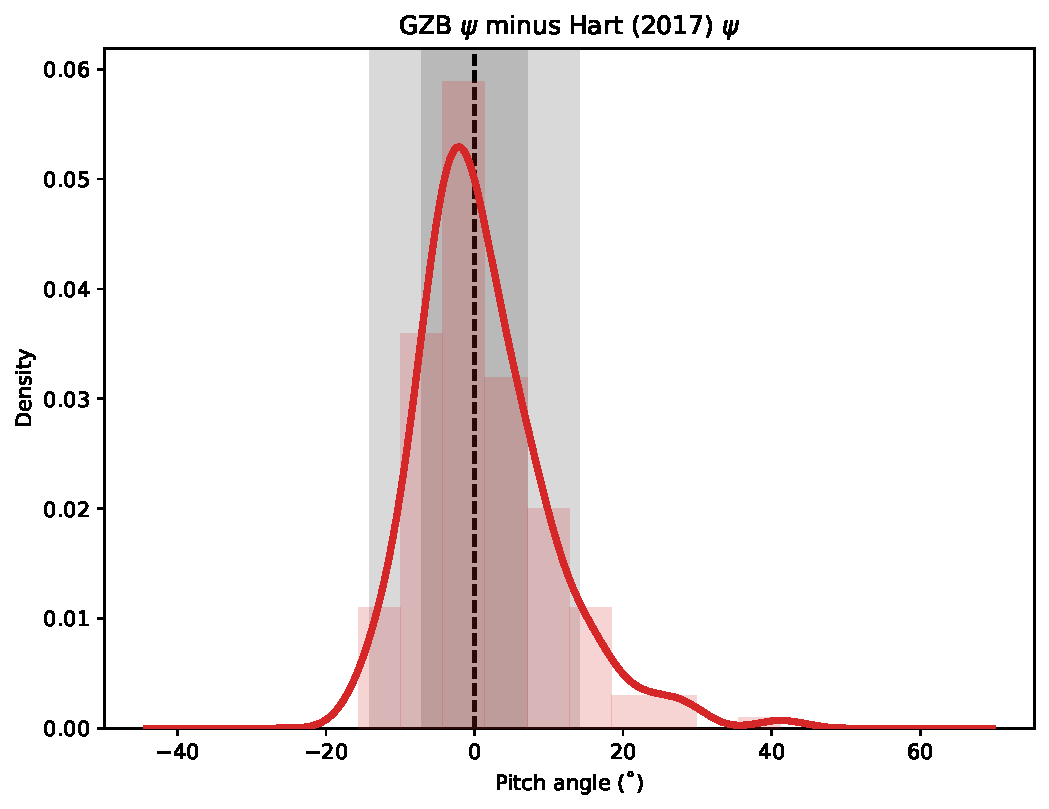
\includegraphics[width=8cm]{images__results/gzb-hart-comparison.pdf}
  \caption{A comparison of Pitch angle obtained by \citet{Hart2016:1607.01019v1} with measured pitch angles for the aggregated model results in galaxies in the Galaxy Zoo Builder sample. The grey regions show 1- and $2\sigma$ errors from \citet{Hart2016:1607.01019v1}. Errors on \textit{Galaxy Builder}-measured pitch angles are not accounted for.}
  \label{fig:hart_pitch_angle}
\end{figure}

\end{document}
